\subsection{Uni-element rocket injector}
%%%%%%%%%%%%%%%%%%%%%%%%%%%%%%%%%%%%%%%%

\begin{figure}[H]
    \centering
    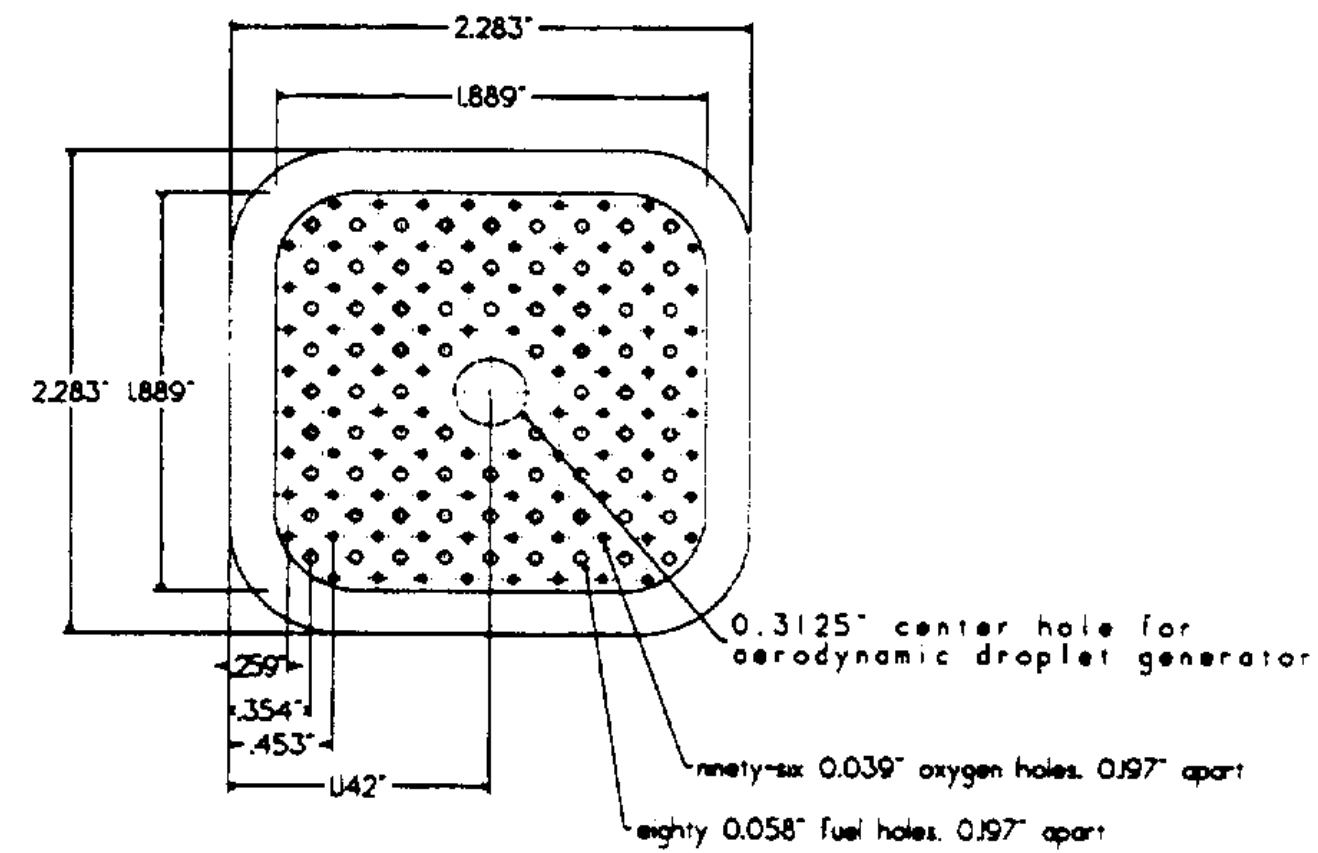
\includegraphics[width=0.35\linewidth]{figs/CCL/fig0.png}
    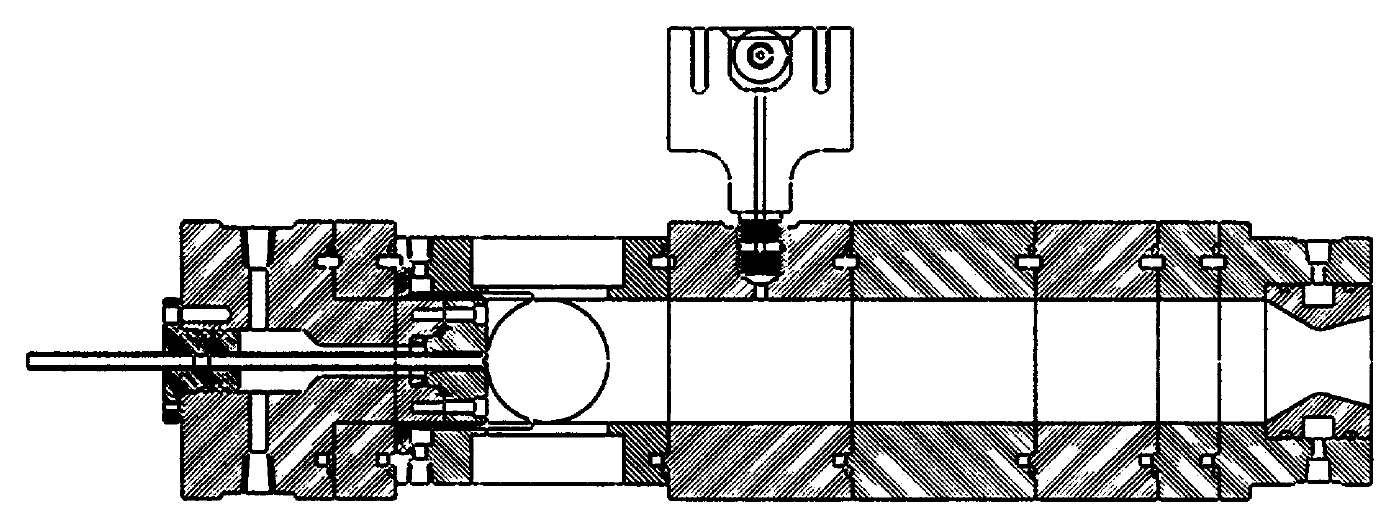
\includegraphics[width=0.5\linewidth]{figs/CCL/fig2a.png}
    \caption{Schematic of the optically-accessible rocket chamber. The chamber is designed such that optical access can be gained for any axial location by interchanging sections. From~\cite{santoro1997experimental, santoro1999main}.}
    \label{fig:enter-label}
\end{figure}

\begin{figure}[H]
    \centering
    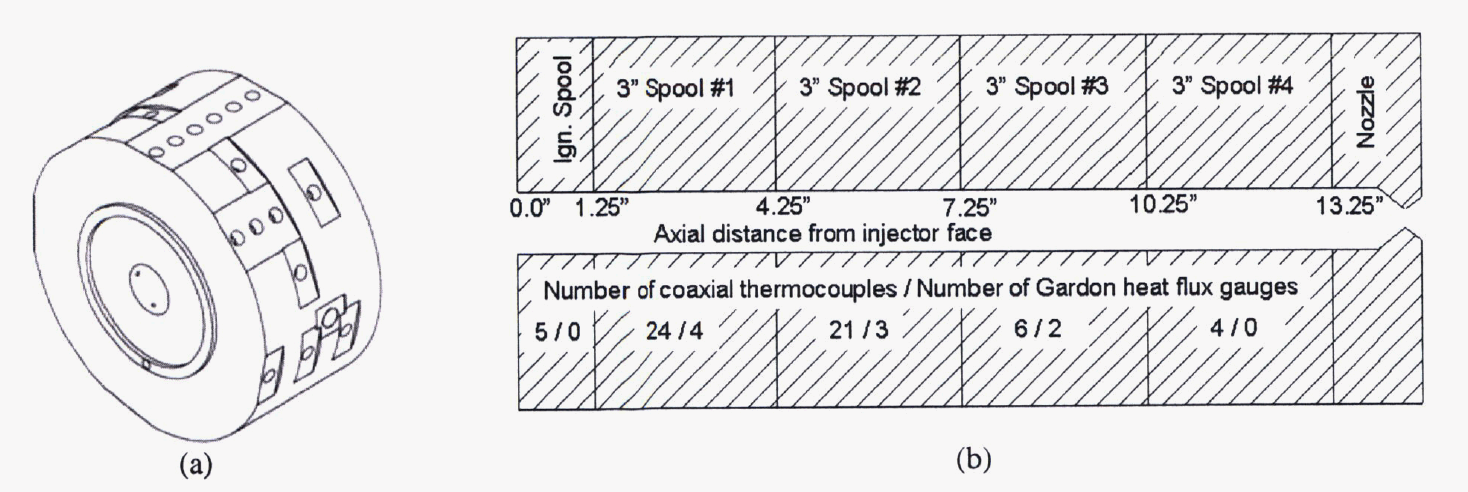
\includegraphics[width=\linewidth]{figs/CCL/fig4.png}
    \caption{(a) Isometric view of combustion chamber spool piece, showing typical locations for instrumentation. (b) Combustion chamber cross section, listing typical instrumentation in each spool piece. From~\cite{jones2006local}.}
    \label{fig:enter-label}
\end{figure}

\begin{figure}[H]
    \centering
    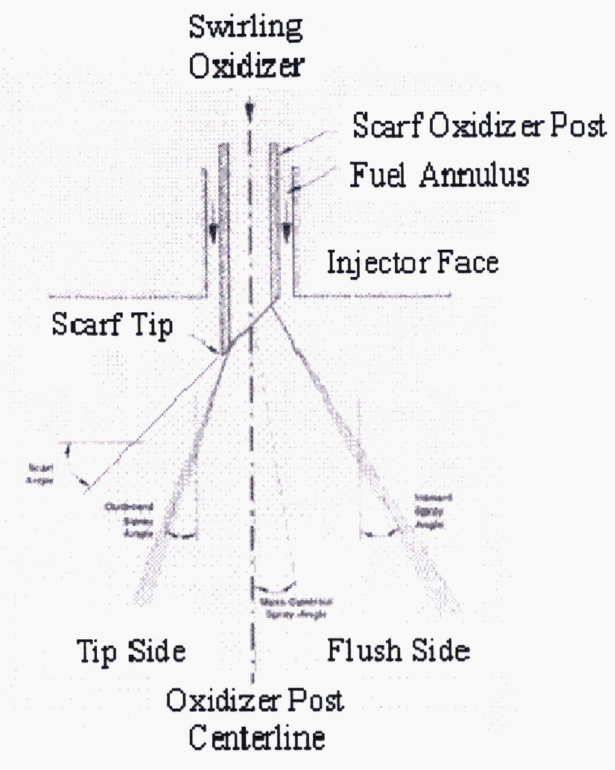
\includegraphics[width=\linewidth]{figs/CCL/fig14.png}
    \caption{Scarf swirl element nomenclature. From~\cite{jones2006local}.}
    \label{fig:enter-label}
\end{figure}
